\documentclass{article}
\usepackage{graphicx}
\usepackage[margin=1in]{geometry}
\usepackage{minted}
\usepackage{amsmath}
\usepackage{mathtools}

\begin{document}

\title{CS102: Objects}

\maketitle
\section{Point}
\subsection{Extend the Point Class}
Using the point class described in class, add the following methods:
\begin{description}
	\item [void display()] prints out \texttt{Point(x, y)}
	\item[string quadrant()] returns the quadrant (Origin, X-Axis, Y-Axis, I, II, III, IV) in which the point lies.
	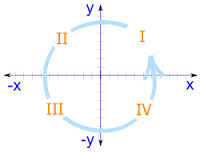
\includegraphics[width=.25\textwidth]{images}
	\item[int above(Point P)] checks if the point calling the function is above the point. \\ For example, given P1.above(P2), the method should return: -1 = $\frac{P2}{P1}$, 0 = P1P2 or P2P1, 1 = $\frac{P1}{P2}$
	\item[int toRight(Point P)] checks if the point calling the function is to the right of the point P.\\ 
For example, given P1.toRight(P2), the method should return: -1 = P1P2, 0 = $\frac{P2}{P1}$ or $\frac{P1}{P2}$, 1 = P2P1
	
\end{description}
\section{Line}
\subsection{Line Functions}
Write a program that includes and uses the following functions:
\begin{description}
	\item[double slope(Point P1, Point P2)] compute the slope of the line that intersects P1 and P2
	\item[double intercept(Point P1, Point P2)] compute the y intercept of the line that intersects P1 and P2
\end{description}

\subsection{Line Class}
Write a line class using the following declaration and a program to test the class. 
\begin{minted}{c++}
class Line{
	public: 
		double slope;
		double intercept;
		Line(Point P1, Point P2);
		//returns true if the line intersects the point
		bool intersects(Point P);
};
\end{minted}
\break
\section{Account}
\subsection{Account Class: Public}
Using this declaration of the account class:
\begin{minted}{c++}
class Account{
    public:
        std::string accountNum;
        double balance;
}
\end{minted}
\begin{description}
    \item[implement the constructor:]Account(std::string name, double b) 
    \item[print out the following in main:] ''Account number: \textit{accountNum} Balance: \textit{balance}''
\end{description}

\subsection{Account Class: Private}
Using this declaration of the account class:
\begin{minted}{c++}
class Account{
    public:
        Account(std::string name, double b);
    private:
        std::string accountNum;
        double balance;
};
\end{minted}
implement the following methods:
\begin{description}
    \item [Account(std::string name, double b)]
        constructor
    \item [void display()]
     prints out ''Account number: \textit{accountNum}
     Balance: \textit{balance}''
    \item[changeBalance(double amount)]
    change the balance by the amount and throw an error if the amount
    is greater than the balance
\end{description}

\subsection{Operator Overloading}
Overload the following operators in the account class described above (private):
\begin{description}
    \item[==] check if two accounts are equal
    \item[\textless\textless]  display the object data using cout and other streams
\end{description}

\subsection{History}
Add the following to the account class described above as private attributes:
\begin{description}
    \item[std::vector \textless double\textgreater history;] attribute to record the history
    \item[displayHistory()] print out the elements in history
    \item[updateHistory(double transaction)] method to add new
    entries. History[0] is the newest transaction.
\end{description}
 
\subsection{Merge}
Add the following method to the account class described above(private):
\begin{description}
    \item[merge(Account B)] merges the balance from B into A
\end{description}

\subsection{Friend Function}
Implement a friend function to merge two accounts into a new account.
Use the following declaration and constructors:
\begin{minted}{c++}
class Account{
    public:
        Account();
        Account(std::string name, double b);
        double getBalance();
        friend Account merge(std::string name, Account a1, Account a2);
    private:
        std::string accountNum;
        double balance;
};
Account::Account(){
}
Account::Account(std::string name, double b){
    accountNum = name;
    balance = b;
}
\end{minted}
Test your function using the following statements in main:
\begin{minted}{c++}
string n1 = ''1234'';
string n2 = ''3245'';
Acount test1(n1, 200);
Account test2(n2, 300);
Account testMerge = merge(''2334'', test1, test2);
cout<<testMerge.accountNumber<<'' ''<<testMerge.getBalance()<<endl;
\end{minted}
\end{document}
